%-----------------------------------------------------------------------------------------------------------------------------------------------------------------------------------------------
% Embasamento Teórico ou Fundamentação Teórica: revisão da literatura dos tópicos que sustentam a ciência e o conhecimento, relativos aos objetivos e aos métodos escolhidos para o desenvolvimento do trabalho.
% Itens como Considerações Iniciais e Finais não são obrigatórios, mas completam muito bem qualquer capítulo.
\chapter{Fundamentos Teóricos}
\label{Revisão Bibliográfica}

A visão estéreo possibilita a identificação de um espaço tridimensional, visto que sua estrutura permite a triangulação de pontos chaves, assim determinando o seu correto posicionamento. Deste modo, compreende-se o porquê deste sistema visual ser amplamente difundido na evolução humana e animal. Em visão computacional, deseja-se emular os sistemas de visão mais eficientes para identificação de objetos e reconhecimento de ambientes. Este processo pode ser realizado  computacionalmente, porém com alguns conceitos como Triangulação, Geometria Epipolar, Calibração e Retificação e Correspondência Estéreo. Estes conceitos encontram-se apresentados nas próximas seções.


%-----------------------------------------------------------------------------------------------------------------------------------------------------------------------------------------------
\section{Visão Estéreo - \textit{Stereo Vision}}
\subsection{Triangulação - \textit{Triangulation}}

Idealmente, a triangulação de um ponto P de coordenadas globais $(X,Y,Z)$ pode ser realizada caso tenha-se uma estrutura estéreo, cujas lentes não apresentem distorção e estejam perfeitamente alinhadas. Deste modo, matematicamente, é possível abstrair os sensores das câmeras como dois planos coplanares entre si. Nessas condições, tem-se que os eixos ópticos das câmeras são paralelos. O eixo óptico, também conhecido como raio principal, é a reta que intercepta o ponto de centro de projeção ${O}$ e o ponto principal da lente ${c}$. Assumindo que as câmeras sejam exatamente iguais e alinhadas, tem-se que os pontos focais da câmera esquerda e da câmera direita são iguais ${f_l = f_r}$ e os pontos principais ${c^{left}_x}$ e  ${c^{right}_x}$ apresentam as mesmas coordenadas \cite{Bradski2008}. A figura \ref{stereo_image_geometric_model} ilustra a representação do modelo idealizado de um sistema estéreo.

\begin{figure}[H]
 	\centering
 	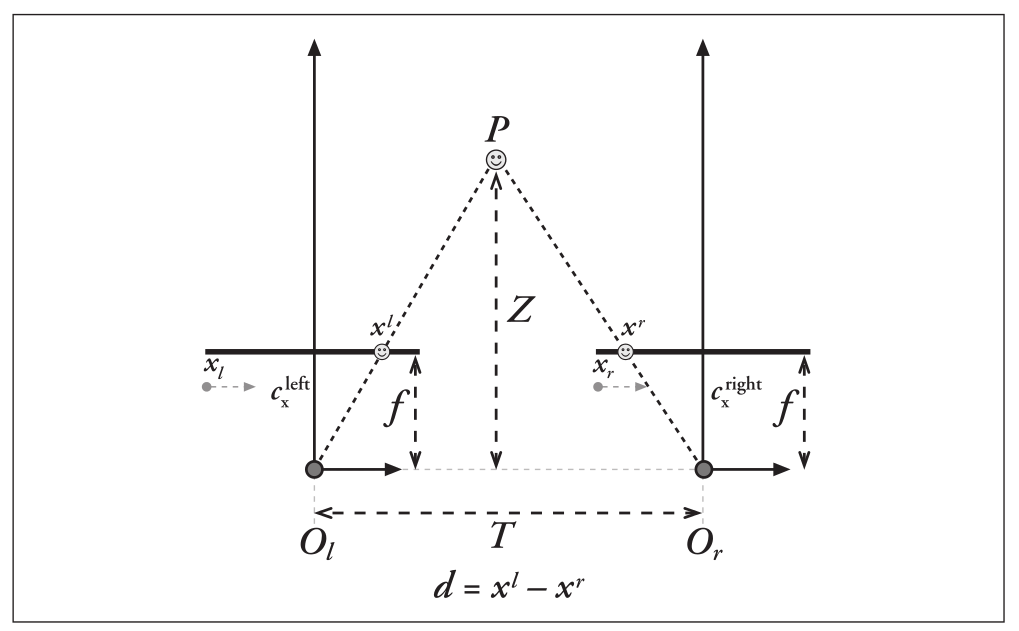
\includegraphics[scale=0.35]{./Resources/bradski/stereo_image_geometric_model.png}
 	\caption{Modelo Idealizado de um sistema de visão estéreo. Imagem retirada de \cite{Bradski2008}}
 	\label{stereo_image_geometric_model}
\end{figure}

A distância presente entre os pontos $x^l$ e $x^r$ é dada pela equação $d = x^l - x^r$, o valor de $d$ é comumente também de chamado de disparidade. Caso os pontos $x^l$ e $x^r$, a distância focal $f$, a distância entre os centros das câmeras $(T,baseline)$ sejam conhecidos é possível determinar a distância entre o ponto P à base das câmeras $(Z)$. Por meio de semelhanças de triângulos, é possível estabelecer uma relação entre os triângulos $O_lPO_r$ e $x^lPx^r$, a qual está apresentada na equação \ref{triangle_similarity}.

\begin{equation}
\label{triangle_similarity}
\frac{T - (x^l-x^r)}{Z-T} = \frac{T}{Z} \Rightarrow Z = \frac{fT}{(x^l-x^r)} = \frac{fT}{d}
\end{equation}


%-----------------------------------------------------------------------------------------------------------------------------------------------------------------------------------------------
\subsection{Geometria epipolar - \textit{Epipolar Geometry}}

Geometria epipolar corresponde à estrutura básica de um sistema estéreo, na qual leva em consideração os modelos \textit{pinhole} de ambas câmeras utilizadas e encontra-se ilustrada pela figura \ref{geometry_epipolar}. 

\begin{figure}[H]
 	\centering
 	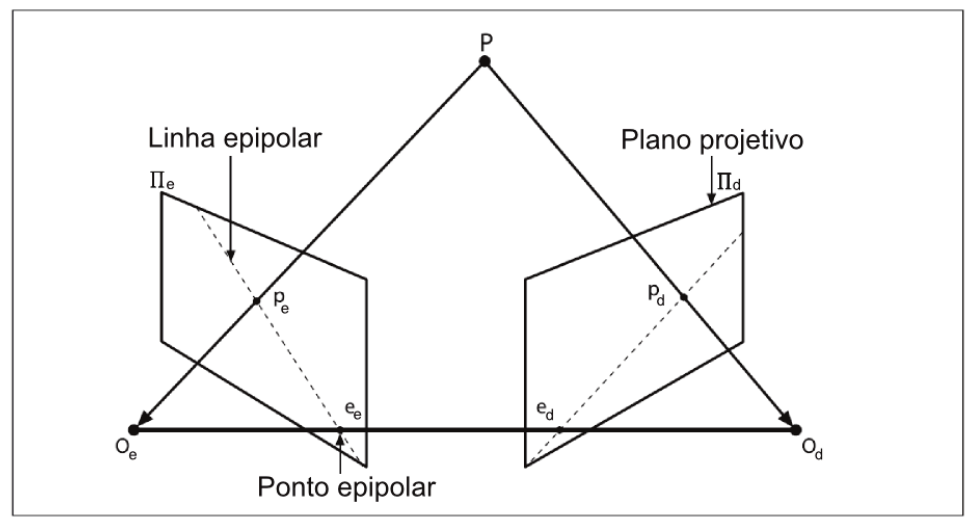
\includegraphics[scale=0.35]{./Resources/bradski/geometry_epipolar.png}
 	\caption{Geometria Epipolar. Imagem retirada de \cite{Mendes2012}}
 	\label{geometry_epipolar}
\end{figure}

Projeta-se o ponto P nos centros de projeção $O^e$ e $O^d$, as linhas que interligam o ponto P a esses centros interceptam os planos $\Pi_e$ e $\Pi_d$ nos pontos $p_e$ e $p_d$. Os pontos epipolares (\textit{epipoles}) $e_e$ e $e_d$ estão localizados nos pontos de intersecção da linha que interliga os centros de projeção e os planos projetivos \cite{Mendes2012}. O conhecimento desta geometria é importante pra o entendimento da chamada restrição epipolar (\textit{epipolar constraint}).

Considerando um sistema estéreo e um certo ponto $P$, deseja-se localizar na imagem da direita o seu ponto homólogo $P'$, isto é, sua projeção no plano projetivo direito. Sem a restrição, faz-se necessário a busca bidimensional em todo espaço do plano $\Pi_d$. Por outro lado, essa restrição garante que o ponto homólogo deve estar sobre a linha epipolar da imagem direita. Deste modo, é possível restringir a busca a uma única dimensão, busca somente sobre a linha epipolar, reduzindo consideravelmente o custo computacional \cite{Bradski2008}. Todavia, o sistema estéreo deve estar corretamente calibrado para que possa tomar mão desta restrição. Em visão computacional, a chamada matriz fundamental refere-se a matrix 3x3 utilizada para relacionar os pontos correspondentes do par de imagens estéreo. A expressão \ref{epipolar_constraint} que representa a restrição epipolar é dada pela relação entre a matriz fundamental F e os dois pontos correspondentes, em coordenadas de pixel \cite{RobertLaganiere}.

\begin{equation}
 \label{epipolar_constraint}
 p'^TFp = 0
\end{equation}


%-----------------------------------------------------------------------------------------------------------------------------------------------------------------------------------------------
\subsection{Calibração das Câmeras - \textit{Calibration}}
\label{theory_calib}

Até o presente momento, todos os conceitos apresentados assumiam que as câmeras são idealmente alinhadas e que suas lentes não apresentavam distorção. Na realidade, os centros ópticos não são perfeitamente alinhados e a lente introduz distorções à imagem projetada no sensor da câmera. Deste modo, faz-se necessário o processo de calibração, o qual mensura estas deformidades e estima os parâmetros que consigam anular ou minimizar estas imperfeições. Isso permite que os métodos computacionais obtenham resultados mais precisos. Estes parâmetros são classificados em dois tipos específicos: intrínsecos e extrínsecos.


%----------------------------------------------------------------------------------------------------------------------------------------------------------------------------------------------
\subsubsection{Parâmetros intrínsecos}

Correspondem às propriedades intrínsecas de cada câmera, as quais são descritas pela matriz M (\textit{Intrinsic Matrix}) e o vetor D (\textit{Distortion Coefficients Vector}). A figura \ref{lenses_distortion} ilustra o modelo completo, componente radial e componente tangencial do modelo de distorções das lentes da câmera esquerda e direita, respectivamente \cite{OpenCVCalibrationModule}.

\begin{equation}
 M = \begin{pmatrix}
f_x & 0   & c_x\\ 
  0 & f_y & c_y\\ 
  0 & 0   & 1
\end{pmatrix}
\end{equation}

\begin{center}
  $f_x,f_y$: Distância focal
  
  $c_x,c_y$: Compensação do ponto principal
\end{center}

\begin{equation}
  D = (k_1,k_2,p_1,p_2[,k_3[,k_4,k_5,k_6]])
\end{equation}

\begin{center}
  $k_1,k_2,k_3$: Coeficientes de distorção radial simétrica
  
  $p_1,p_2$: Coeficientes de distorção tangencial (descentrada)
\end{center}

%----------------------------------------------------------------------------------------------------------------------------------------------------------------------------------------------
\subsubsection{Parâmetros extrínsecos}
Correspondem às propriedades extrínsecas, isto é, demonstram a disposição espacial da segunda câmera, direita, com relação à câmera da esquerda em coordenadas globais. Assim como ilustrado na figura \ref{essential_geometry.png}, a matriz de rotação R (3x3) e o vetor de translação T (3x1) são responsáveis por descrever este deslocamento. Geralmente, quando o quadro de referência não se encontra no centro de projeção da câmera, faz-se necessário a adição da matriz de rotação e o vetor de translação. Neste contexto, utiliza-se o sistema de coordenadas homogêneas, isto é, pontos 2D são representados como vetores 3x1 e pontos 3D como vetores 4x1. Deste modo, tem-se que a equação \ref{projection_equation} descreve a relação do ponto $P(X,Y,Z)$ e o ponto projetado $p'$ no plano $\Pi_r$\cite{RobertLaganiere}.

%----------------------------------------------------------------------------------------------------------------------------------------------------------------------------------------------
\begin{equation}
  s.p' = M
  \begin{bmatrix}
  \begin{array}{c|c}
  R & t
  \end{array}
  \end{bmatrix}
  P 
\end{equation}

%----------------------------------------------------------------------------------------------------------------------------------------------------------------------------------------------
\begin{equation}
\label{projection_equation}
s
\begin{bmatrix}
x \\ 
y \\ 
1 
\end{bmatrix}
= 
\begin{bmatrix}
f_x & 0 & c_x\\ 
0 & f_y & c_y\\ 
0 & 0 & 1
\end{bmatrix} 
\begin{bmatrix}
r_{11} & r_{12} & r_{13} & t_1 \\ 
r_{21} & r_{22} & r_{23} & t_2 \\ 
r_{31} & r_{32} & r_{33} & t_3
\end{bmatrix}
\begin{bmatrix}
X \\ 
Y \\ 
Z \\ 
1
\end{bmatrix}
\end{equation}

%----------------------------------------------------------------------------------------------------------------------------------------------------------------------------------------------
\begin{figure}[H]
 	\centering
 	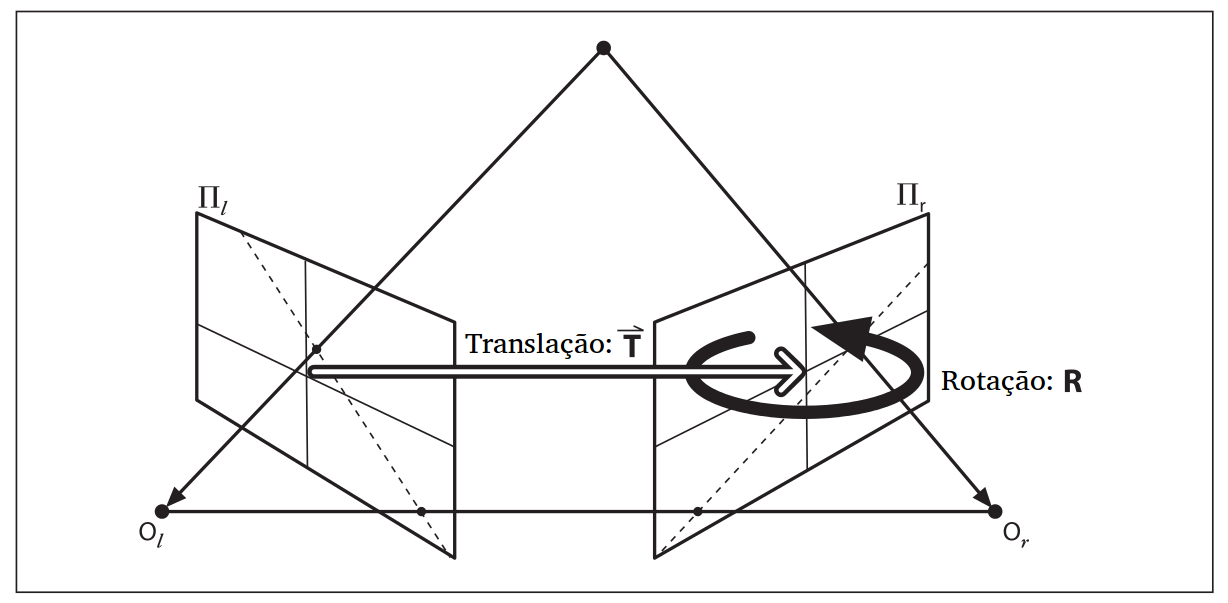
\includegraphics[scale=0.25]{./Resources/bradski/essential_geometry_ptbr.png}
 	\caption{O deslocamento do plano $\Pi_r$ com relação ao plano $\Pi_l$ pode ser descrito pela matriz R e o vetor de translação T. Imagem retirada de \cite{Bradski2008}.}
 	\label{essential_geometry.png}
\end{figure}

%----------------------------------------------------------------------------------------------------------------------------------------------------------------------------------------------
Devido ao desalinhamento entre as câmeras, torna-se necessário estimar estas variáveis, aumentando, assim, a eficiência dos métodos estéreo ao procurarem pelas correspondências entre as duas imagens. A figura \ref{stereo_calib_extrinsic}, ilustra o processo de calibração dos parâmetros extrínsecos, no qual utiliza-se um conjunto de imagens do padrão de calibração. Ao fim deste processo, é possível aferir o posicionamento da segunda câmera com relação à primeira \cite{Bouguet1999}.


%----------------------------------------------------------------------------------------------------------------------------------------------------------------------------------------------
\subsection{Retificação das Imagens - \textit{Rectification}}

O processo de retificação é responsável por realizar as correções com relação à distorção das lentes e ao alinhamento das câmeras, de acordo com os parâmetros obtidos pelo processo de calibração apresentado no tópico anterior. Ao fim deste processo, deseja-se que o par de imagens estéreo esteja retificado e sem distorções, preparado para a aplicação dos métodos estéreo, assim como ilustrado na figura \ref{rectification_process}.

\begin{figure}[H]
 	\centering
 	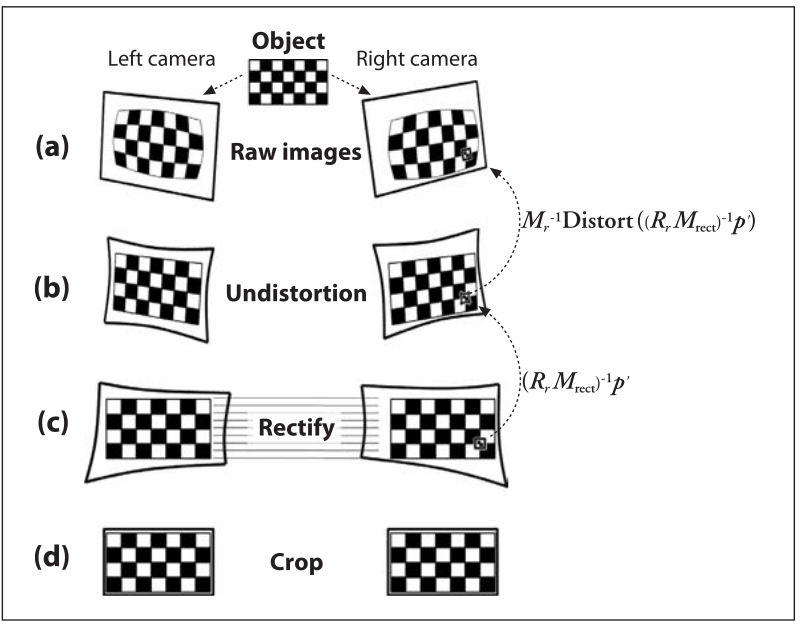
\includegraphics[scale=0.32]{./Resources/bradski/rectification_process.png}
 	\caption{Retificação de Imagens - Processo de retificação estéreo. Imagem retirada de \cite{Bradski2008}.}
 	\label{rectification_process}
\end{figure}


%-----------------------------------------------------------------------------------------------------------------------------------------------------------------------------------------------
\subsection{Correspondência Estéreo - \textit{Stereo Correspondence}}

Correspondência estéreo não é nada mais que a utilização de métodos estéreo, os quais são responsáveis pela procura de pontos homólogos nos pares de imagens estéreo. Como visto anteriormente, devido ao distanciamento das câmeras $(T)$ e ao distanciamento do objeto com relação às câmeras $(Z)$, o mesmo ponto apresenta diferentes posicionamento nos planos das câmeras $x^l$ e $x^r$. A figura \ref{homologous_points _stereo} ilustra um par de imagens estéreo (esquerda e direita) e o mapa de disparidades gerado pela cena, nas quais os pixels homólogos estão destacados. Os métodos estéreo utilizam da restrição epipolar o que reduz o espaço de busca e de diferentes meios para encontrá-los. Mesmo com essa restrição e com a retificação das imagens, os métodos ainda assim apresentam um elevado custo computacional, além do que ainda estão sujeitos à encontrarem falsas correspondências. 

\begin{figure}[H]
 	\centering
 	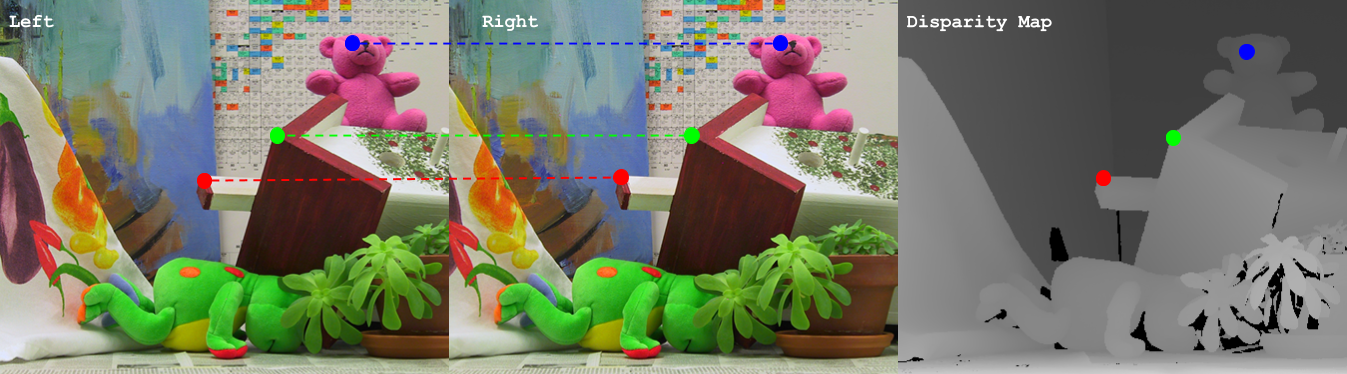
\includegraphics[scale=0.33]{./Resources/homologous_points_stereo.png}
 	\caption{Correspondência de pontos homólogos em um par de imagens estéreo. Imagem original retirada de \cite{Scharstein2003}.}
 	\label{homologous_points _stereo}
\end{figure}


%-----------------------------------------------------------------------------------------------------------------------------------------------------------------------------------------------
\subsubsection{Mapa de disparidades - \textit{Disparity Map}}

Como já foi dito anteriormente, disparidade é o deslocamento dos pontos homólogos entre as duas imagens. Nos métodos estéreo, o valor da disparidade é codificado em escala de cinza, a qual é inversamente proporcional à distância do objeto, assim como representado na figura \ref{depth_disparity}. Assim, níveis de cinza mais altos (tons claros) correspondem a disparidades maiores (perto) e níveis de cinza mais baixos (tons escuros) correspondem a disparidades mais baixas (distante). Devido a sua relação com a distância, este conceito é comumente atrelado à percepção de profundidade.

\begin{figure}[H]
 	\centering
 	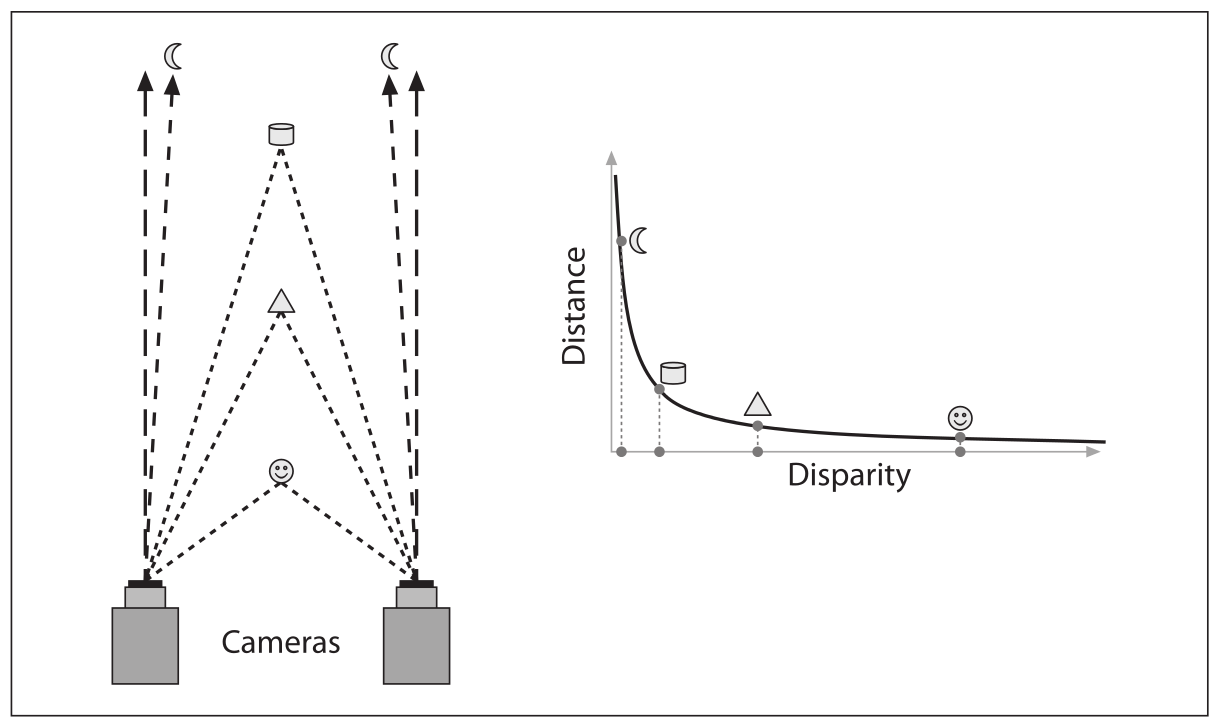
\includegraphics[scale=0.3]{./Resources/bradski/depth_disparity.png}
 	\caption{Relação inversamente proporcional entre distância e disparidade. Imagem retirada de \cite{Bradski2008}}
 	\label{depth_disparity}
\end{figure}

%-----------------------------------------------------------------------------------------------------------------------------------------------------------------------------------------------
\subsubsection{Métodos Estéreo}
\label{stereo_methods}
A seguir, encontra-se apresentado um pequeno resumo de como são os operadores dos métodos estéreo utilizados neste trabalho.

\begin{enumerate}
 \item \textbf{\textit{Block Matching} - BM:} Este algoritmo é um método local, no qual utiliza soma das diferenças ao quadrado (SSD - \textit{Sum of Squared Differences}) para a determinação de correspondências. O tamanho da vizinhança deve ser avaliado, visto que a densidade do mapa gerado, nível de detalhamento e intensidade de ruído dependem disso. Caso o bloco seja pequeno, o mapa apresentará detalhes mais nítidos, porém adicionará ruídos ao mapa. Por outro lado, um bloco maior reduz o nível de ruído, porém diminui o nível de detalhamento do mapa. As limitações serviram de motivação para a criação do método a seguir \cite{Hirschmuller2008}.   

 \item \textbf{\textit{Semi-global Block Matching} - SGBM:} Este algoritmo é um método global e também visa a obtenção de uma correspondência estéreo mais precisa, para isso, além da etapa de agregação de custo (cálculo da similaridade), modela-se o sistema como um problema de minimização energética, o que adiciona restrições que suavizam o mapa ao penalizar descontinuidades.  \cite{JunhwanKim2003}. Por conta disso, este método é mais lento que o apresentado anteriormente, porém é mais denso ao comparar-se o nível de detalhamento para um bloco de tamanho pequeno \cite{Hirschmuller2008}.

 \item \textbf{\textit{Block Matching with GPU Acceleration} - BMGPU:} Método é igual ao primeiro apresentado, diferindo do fato que as suas bibliotecas e métodos implementados são voltados para a aceleração em GPU (\textit{Graphics Processing Unit}). Dado o paralelismo inerente dos aceleradores gráficos de hoje, esse tipo de \textit{hardware} permite o processamento simultâneo dos dados. 
\end{enumerate}


%-----------------------------------------------------------------------------------------------------------------------------------------------------------------------------------------------
\subsection{Aplicações em Robótica}
\label{aplicacoes_robotica}
Nesta seção, serão apresentados alguns dos trabalhos que têm como principais sensores câmeras estéreo para a navegação autônoma em ambientes terrestre, aérea e subaquática.

Nos dias de hoje, as empresas automobilísticas vêm participando de uma verdadeira corrida tecnológica para o desenvolvimento de automóveis totalmente autônomos e economicamente viáveis. As universidades não ficaram para trás e também apresentam pesquisas envolvendo desenvolvimento de algoritmos de controle e sensores, tornando essa corrida ainda mais acirrada. Os resultados apresentados são realmente promissores, e concretizam cada vez mais essa realidade tida até então como distante. Na figura \ref{caminhao_autonomo}, é possível observar o projeto de caminhão autônomo desenvolvido pelo Laboratório de Robótica Móvel - LRM - ICMC/USP. O caminhão conta com diversos sensores, dentre eles câmeras estéreo, que identificam outros automóveis, pessoas e faixas de sinalização \cite{ShinzatoP}. 


%-----------------------------------------------------------------------------------------------------------------------------------------------------------------------------------------------
\begin{figure}[H]
 	\centering
 	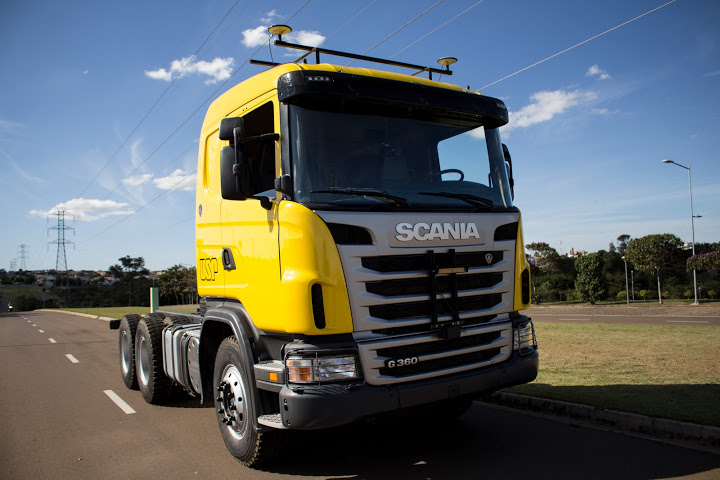
\includegraphics[scale=0.40]{./Resources/caminhao_autonomo.jpg}
 	\caption{Caminhão Autônomo desenvolvido pelo Laboratório de Robótica Móvel - LRM - ICMC/USP em parceria com a Scania.}
 	\label{caminhao_autonomo}
\end{figure}


%-----------------------------------------------------------------------------------------------------------------------------------------------------------------------------------------------
No caso de navegação autônoma para ambiente aéreo, o projeto utilizando \textit{Micro Air Vehicle} (MAVS) desenvolvido pelo \textit{Massachusetts Institute of Technology} (MIT) permite que pequenas aeronaves consigam navegar autonomamente e desviar de obstáculos voando a uma velocidade de 30 mph (48 $km/h$). A figura \ref{mit_drones} apresenta o trabalho desenvolvido, o qual é um comparativo de desempenho de uma implementação em hardware utilizando \textit{Field-programmable gate array} (FPGA) e um processador ARM para processamento embarcado do método SGBM \cite{BarryMIT}.


%-----------------------------------------------------------------------------------------------------------------------------------------------------------------------------------------------
\begin{figure}[H]
 	\centering
 	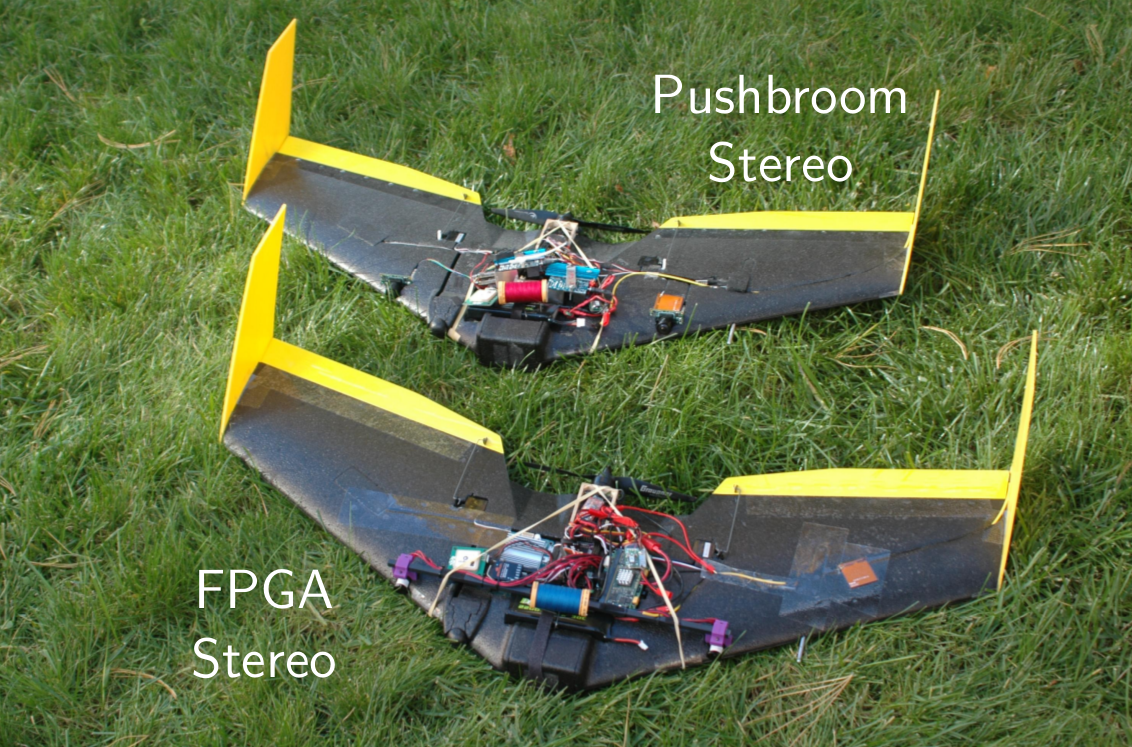
\includegraphics[scale=0.26]{./Resources/mit_drones.png}
 	\caption{Plataformas experimentais de aeronaves com o Sistema Estéreo - FPGA e o Sistema Estéreo - Pushbroom. Câmeras são montados na parte dianteira das asas na mesma linha de base (34 cm) em ambas células. Imagem retirada de \cite{BarryMIT}.}
 	\label{mit_drones}
\end{figure}


%-----------------------------------------------------------------------------------------------------------------------------------------------------------------------------------------------
No caso de navegação autônoma para ambiente subaquático, um exemplo de \textit{autonomous underwater vehicle} (AUV) é o projeto desenvolvido pela Universidade espanhola de Girona (veja figura \ref{G500}). O trabalho propõe a utilização do método de Mapeamento e Localização Simultânea (SLAM), juntamente com câmera estéreo, para o reconhecimento do ambiente, aprimorando assim o erro de rastreamento dos objetos \cite{Nagappa2013}.


%-----------------------------------------------------------------------------------------------------------------------------------------------------------------------------------------------
\begin{figure}[H]
 	\centering
 	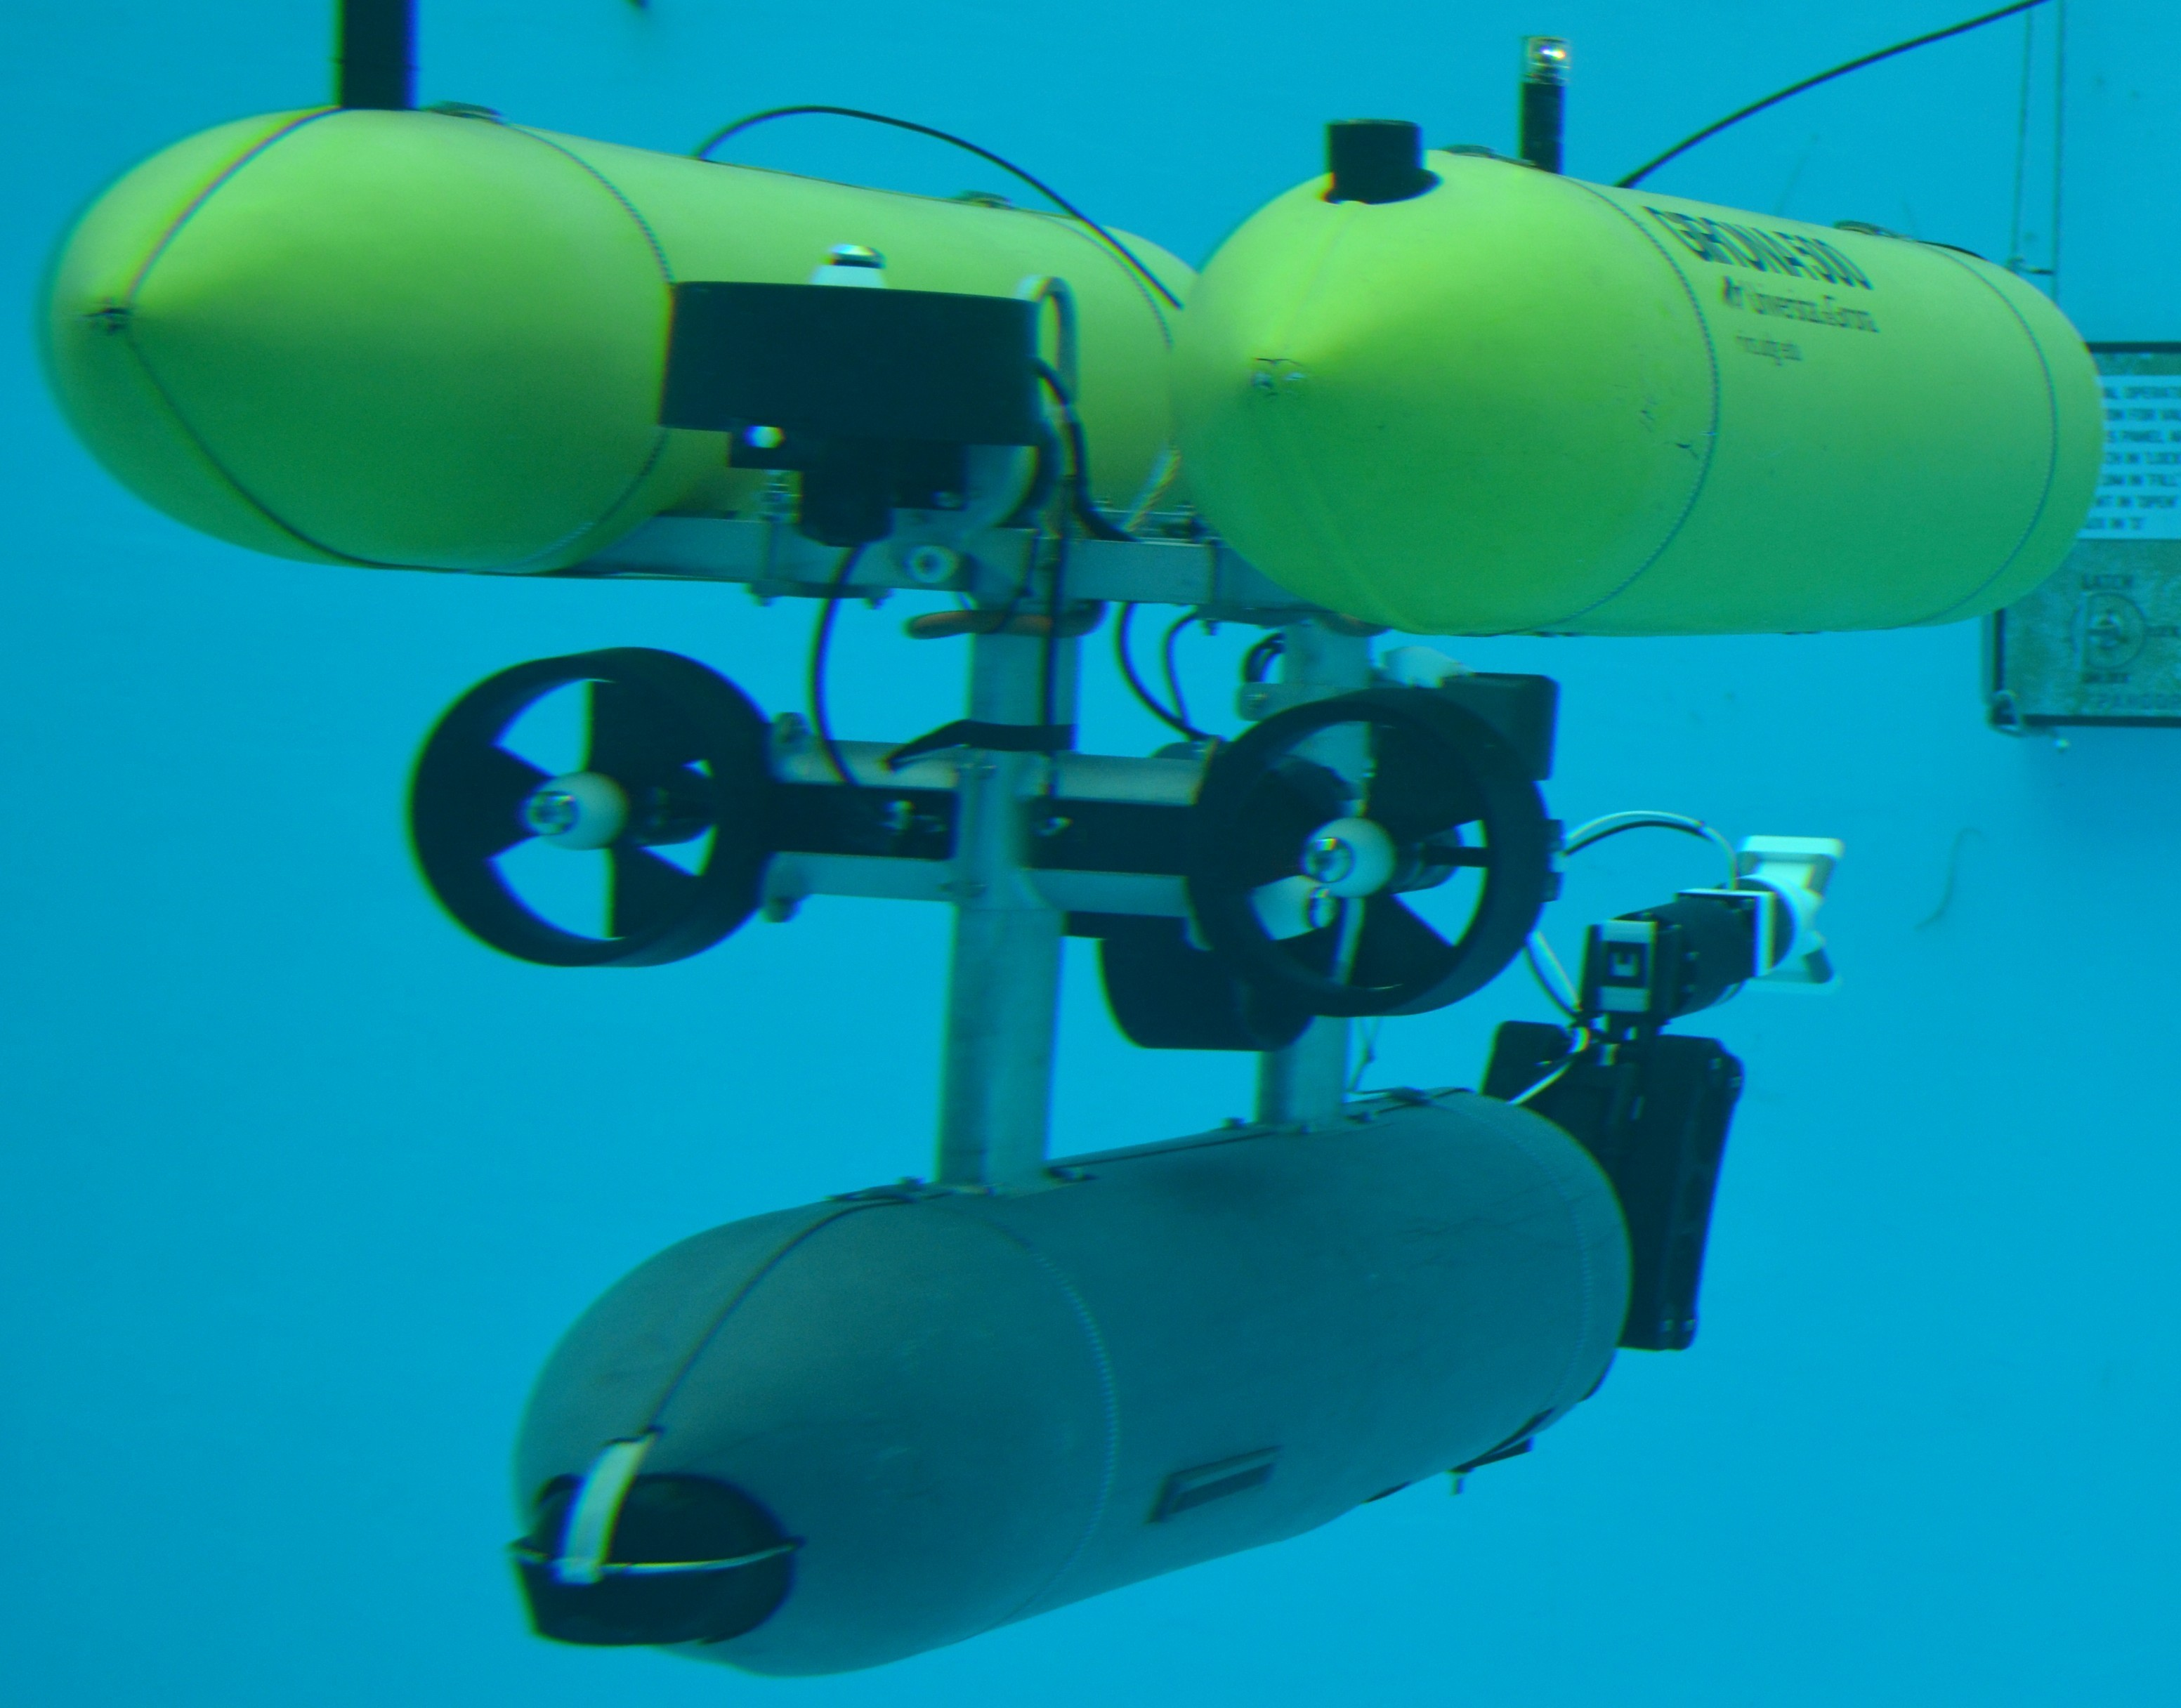
\includegraphics[scale=0.1]{./Resources/G500.jpg}
 	\caption{Veículo Submarino Autônomo - Girona 500}
 	\label{G500}
\end{figure}


%-----------------------------------------------------------------------------------------------------------------------------------------------------------------------------------------------
\section{OpenCV}
\textit{Open Source Computer Vision Library} (OpenCV) é uma biblioteca de código aberto, a qual reúne diversos algoritmos relacionados a visão computacional. O OpenCV foi criado pelo centro de pesquisa da \textit{Intel}, e atualmente é mantido pelo time de pesquisadores da companhia \textit{Itseez} \cite{ItseezOpenCVinfo}. A biblioteca é estruturada em diferentes módulos, os quais agrupam os algoritmos relacionados a tópicos como processamento de imagem, estimativa de movimento, correspondência estéreo, extratores de características, criação de interfaces de usuário e aceleração em \textit{hardware}. O OpenCV foi criado com a intensão de ser multiplataforma, por conta disso, em sua maior parte, foi escrito em linguagem C/C++, o que o torna facilmente portável para diversas plataformas como Windows, Linux, Android, MacOS, iOS, dentre outros. Recentemente, módulos dando suporte à CUDA (seção \ref{cuda}) e OpenGL foram incorporados à biblioteca expandindo ainda mais o número de aplicações possíveis \cite{ItseezOpenCVPlatforms}. 


%-----------------------------------------------------------------------------------------------------------------------------------------------------------------------------------------------
\section{Linux Embarcado}

Linux é um sistema operacional de código-aberto que é amplamente utilizado, cujo \textit{Kernel}, originalmente escrito por Linus Torvalds, pode suportar diversos designs de sistemas podendo ser um computador pessoal, um supercomputador ou \textit{cluster}, ou até mesmo sistemas \textit{System-on-Chip} (SoC). Este sistema é capaz de suportar diversas arquiteturas de processadores como x86{\_}64, PowerPC, ARM, MIPS, StrongARM, XScale, dentre outras \cite{Wang2011}.

A popularização do termo Linux fez com que atualmente exista uma certa confusão sobre a distinção de um \textit{Kernel} de um sistema operacional e do sistema operacional propriamente dito. A maior razão desta confusão é a variedade de distribuições desenvolvidas pela comunidade, visto a facilidade para customizar seus módulos, pacotes, sistemas de arquivo e servidores gráficos. Dada sua versatilidade, logo tornou-se a peça chave para o desenvolvimento de sistemas embarcados, os quais são computadores completamente especializados para a realização de tarefas específicas. Esses sistemas diferem de computadores de propósito geral e comumente apresentam certas restrições de dimensão, condições de operação, ou limitação de recursos computacionais como menor poder de processamento ou menor capacidade de armazenamento. 

Assim, começaram a surgir distribuições de Linux, os chamados \textit{Embedded Linux}, que apresentavam menores requisitos de sistemas, devido à remoção de módulos que não são utilizados em determinados sistemas ou à otimização desses módulos para aquela atividade específica \cite{Yaghmour2008}.


%-----------------------------------------------------------------------------------------------------------------------------------------------------------------------------------------------
\section{Aceleração em Hardware - CUDA}
\label{cuda}

\textit{Compute Unified Device Architecture} (CUDA) é uma tecnologia desenvolvida pela NVIDIA e em sua essência é uma plataforma de computação paralela de propósito geral, cujo objetivo é tirar proveito das unidades de processamento gráfico (GPU), assim, acelerando consideravelmente a execução de algoritmos computacionais complexos ao comparar-se com o desempenho da CPU.

Atualmente, a maioria das placas de vídeo da NVIDIA contam com essa tecnologia, por conta disso os pesquisadores e desenvolvedores de software estão voltando suas pesquisas para o desenvolvimento e otimização de algoritmos que possam explorar todo o poder de processamento destes dispositivos. Alguns exemplos de aplicações são identificação de placas ocultas em artérias, análise do fluxo de tráfego aéreo \cite{Monish2011} e visualização de moléculas \cite{Stone2015}.

Historicamente, a implementação de algoritmos em GPU mostrou-se bastante obscura, visto que sua programação era bastante atrelada ao hardware a ser utilizado, mesmo com linguagens de programação gráfica como o OpenGL. Em 2003, um grupo de pesquisadores de Stanford, apresentou o primeiro compilador, Brook, que facilitaria a implementação de software, visto que permitia lidar de uma maneira mais maleável o fluxo de dados, podendo principalmente paralelizá-los. Em 2006, a NVIDIA juntamente com Ian Buck, criador do Brook, desenvolveu uma plataforma (CUDA) mais intuitiva e que permitisse a utilização de uma linguagem de alto nível e tornasse a GPU em um processador de propósito geral (GPGPU) \cite{NVIDIA}.
